%-------------------------------------------------------------------------------
\section{Motivation}\label{motivation}
%-------------------------------------------------------------------------------

We now explore in further detail the benefits that serverless has to offer, and
the current state of serverless offerings.

\subsection{Benefits of serverless}

The main attraction of serverless for developers is, in an idealized world, the
characteristic of only paying for what they use, while having a whole datacenter
available to them. This proposition is especially attractive to developers of
applications where the amount of resources that they need varies significantly
over time, or is generally small and very spread out. With such workloads,
buying their own machines or renting a fixed amount of server space is bad for
the developer because it is expensive if provisioned for peak usage and has poor
performance if not, and bad for providers becuase it leads to low utilization.

A central example to this paper is that of a web server. Its traffic patterns
make it a great candidate for running as serverless functions: it is
event-based, its load is bursty and unpredictable, and a request's resource
requirements can vary greatly depending on which user invoked it.


A back of the envelope calculation shows that for web servers with small load,
lambda functions as they stand today are cheaper: for a low-traffic website,
with approx 50K requests per day, a memory footprint of < 128 MB, and 200ms of
execution, running that on AWS lambda adds up to \$1.58 per month. On the other
hand, the cheapest EC2 instance costs just over \$3 per month. Of course, as the
number of requests goes up, the price for lambdas scales linearly, whereas
running an EC2 instance on full load becomes comparably cheap. Extensive
simulations show a more nuanced picture of the tradeoff points for different
workloads~\cite{econ-of-serverless,trek10-blog}.

Serverless also may outperform reservation systems for workloads that are very
bursty: starting a new lambda execution environment is much faster than starting
a new container or EC2 instance, which can take multiple
minutes~\cite{ec2-autoscaling}.


\subsection{State of the world}


\begin{figure}[t!]
    \centering
      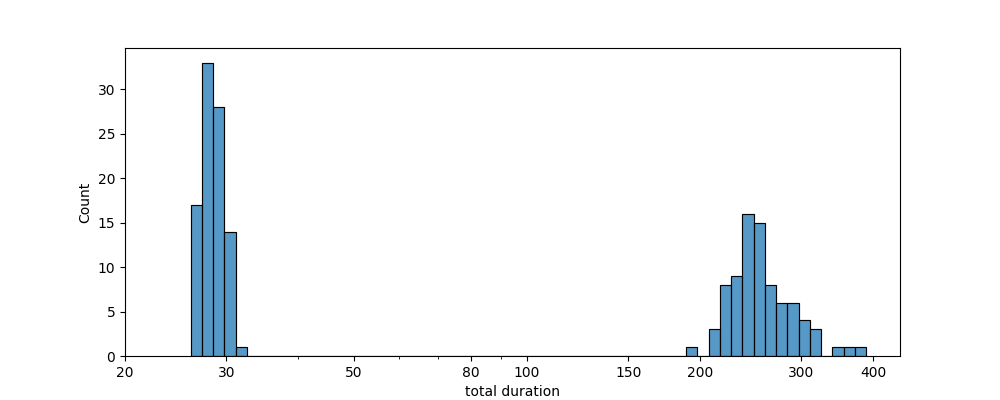
\includegraphics[width=8.5cm]{img/lambda_total_durations.png}
      \caption{ distribution of end to end duration times. The x axis is log scale }
    \label{fig:lambda-total-durations}
\end{figure}

However, only few web servers run entirely on serverless offerings today. There
are many reasons that developers choose not to use serverless, despite their
workloads being well-suited for the serverless
environment~\cite{not-lambda-blog,reddit-serverless2}. Popular complaints
include provider lock in, lack of insight for debugging and telemetry, and
variable runtimes.


\Sys{} focuses on the challenge of variable runtimes. In order to better
understand the where the variation comes from, we run an experiment with a
simple lambda function that sleeps for 20ms and then returns. We use AWS
Xray~\cite{aws-xray} to measure its latency, with incovations spaced randomly
between 0 and 10 minutes. The results are in
Figure~\ref{fig:lambda-total-durations}. We can see that the durations can be
grouped into two categories: cold start and warm start, which we explore
separately.

\textbf{Cold start behavior}.
% 
The right grouping in the graph is those invocations that hit cold starts, whose
overall latencies vary between 200 and 400ms.

\begin{figure}[t!]
  \centering
    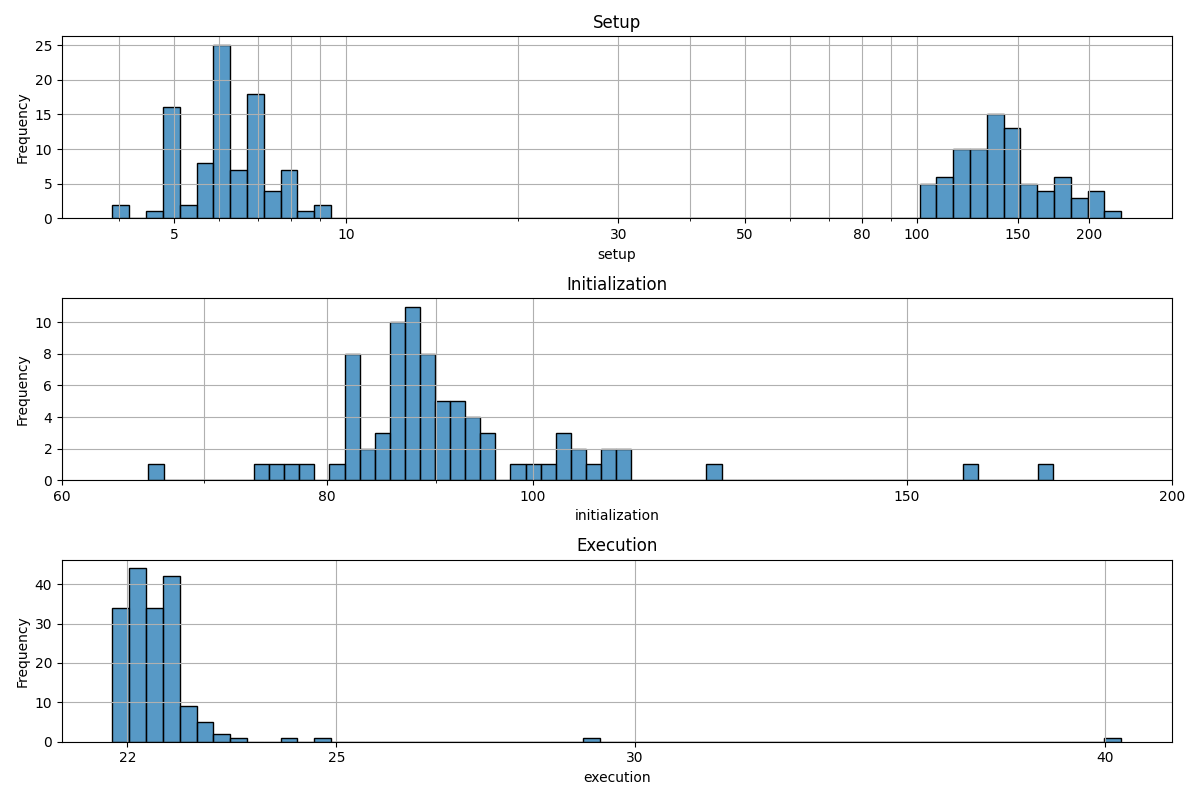
\includegraphics[width=8.5cm]{img/lambda_duration_breakdown.png}
    \caption{ Breakdown of variation in duration times. X axes are all log scale }
  \label{fig:lambda-durations-breakdown}
\end{figure}

In order to better understand where that variability comes from, we look into a
breakdown of the latencies. We are able to break down the total duration into
three components: \textit{setup}, which includes placing the function and
creating the container; \textit{initialization}, which is any code that runs
before the function does, for example initializing the runtime and any python
modules the function uses; and \textit{execution}, actually executing the
functions code. Xray gives us only the latter two values explicitly, we
calculate the setup time by looking at the total duration and subtracting the
initalization and execution times. 

We can see the resulting distributions in
Figure~\ref{fig:lambda-durations-breakdown}, with times from cold start
invocations colored in blue. The most stable component of the duration is the
execution time, although it has some outliers. The initialization time has a
range of $>$100ms, and is only nonzero for cold start invocations. In the setup
times we can see two groupings: warm start on the left that does not include
placing or starting the container, and cold start on the right that does. Warm
invocations' setup has a range of $\sim$5ms, and cold invocations' a range of
$\sim$120ms. Where exactly this range for cold invocations' setup times
comes from is impossible to know without futher insight into the system, but
clear is that sometimes AWS is able to get the cold start container up and
running in just over 100ms, and sometimes it takes as much as $\sim$250ms.


\textbf{Warm start behavior}. 
% 
The times on the left side of the graph in
Figure~\ref{fig:lambda-total-durations} are the execution times from invocations
with warm start. We can see that their durations are comparably stable. The
reason for this is that AWS is able to simply route the new invocation to the
machine with the existing container on it. We verify that this is indeed what is
happening by changing the function to include reading and then writing to an
environment variable, and find that for invocations with warm start when we read
the variable it was already set by a previous invocation.

We extend the experiment to understand whether AWS will also use other functions
containers with the same runtime. We run the following experiment: two different
functions, foo and bar, that both use the same runtime (the AWS Python 3.13
environment), and we use the same trick of reading and then setting an
environment variable to an invocation-specific value. We first run foo once, and
then immediately fire off 100 parallel invocations of bar. Even though many of
the bar invocations experience cold start, those that have warm start are
reusing containers from already completed bar invocations; none of them use the
container created by foo. We can conclude that AWS does not allow a tenant's
different functions to share containers, even if they need the same runtime.

In order to increase the number of warm start experienced, it might seem
desirable to be able to use a different function's warm container. However, that
would require AWS to know which function should have priority over the other in
order to know which to prefer, or whether to preempt, in the case that
invocations of two different functions are competing for the same container.
Instead, AWS offers two different ways for developers to influence their
functions' scaling: provisioned and reserved concurrency\cite{aws-scaling}.
Provisioned concurrency specifies a number of instances to keep warm for a given
function, and reserved concurrency ensures that a fixed amount of the possible
concurrency reserved for it. This interface is bad for serverless workloads for
the same reasons that reservation-based systems are: it requires developers to
estimate their future needs and pay up front, and providers to keep those
potentially idle resources available.





